\documentclass[]{article}
\usepackage{lmodern}
\usepackage{amssymb,amsmath}
\usepackage{ifxetex,ifluatex}
\usepackage{fixltx2e} % provides \textsubscript
\ifnum 0\ifxetex 1\fi\ifluatex 1\fi=0 % if pdftex
  \usepackage[T1]{fontenc}
  \usepackage[utf8]{inputenc}
\else % if luatex or xelatex
  \ifxetex
    \usepackage{mathspec}
  \else
    \usepackage{fontspec}
  \fi
  \defaultfontfeatures{Ligatures=TeX,Scale=MatchLowercase}
\fi
% use upquote if available, for straight quotes in verbatim environments
\IfFileExists{upquote.sty}{\usepackage{upquote}}{}
% use microtype if available
\IfFileExists{microtype.sty}{%
\usepackage{microtype}
\UseMicrotypeSet[protrusion]{basicmath} % disable protrusion for tt fonts
}{}
\usepackage[margin=1in]{geometry}
\usepackage{hyperref}
\hypersetup{unicode=true,
            pdftitle={MovieLens Capstone},
            pdfauthor={Mohammed Amine BOUSSETTA},
            pdfborder={0 0 0},
            breaklinks=true}
\urlstyle{same}  % don't use monospace font for urls
\usepackage{color}
\usepackage{fancyvrb}
\newcommand{\VerbBar}{|}
\newcommand{\VERB}{\Verb[commandchars=\\\{\}]}
\DefineVerbatimEnvironment{Highlighting}{Verbatim}{commandchars=\\\{\}}
% Add ',fontsize=\small' for more characters per line
\usepackage{framed}
\definecolor{shadecolor}{RGB}{248,248,248}
\newenvironment{Shaded}{\begin{snugshade}}{\end{snugshade}}
\newcommand{\KeywordTok}[1]{\textcolor[rgb]{0.13,0.29,0.53}{\textbf{#1}}}
\newcommand{\DataTypeTok}[1]{\textcolor[rgb]{0.13,0.29,0.53}{#1}}
\newcommand{\DecValTok}[1]{\textcolor[rgb]{0.00,0.00,0.81}{#1}}
\newcommand{\BaseNTok}[1]{\textcolor[rgb]{0.00,0.00,0.81}{#1}}
\newcommand{\FloatTok}[1]{\textcolor[rgb]{0.00,0.00,0.81}{#1}}
\newcommand{\ConstantTok}[1]{\textcolor[rgb]{0.00,0.00,0.00}{#1}}
\newcommand{\CharTok}[1]{\textcolor[rgb]{0.31,0.60,0.02}{#1}}
\newcommand{\SpecialCharTok}[1]{\textcolor[rgb]{0.00,0.00,0.00}{#1}}
\newcommand{\StringTok}[1]{\textcolor[rgb]{0.31,0.60,0.02}{#1}}
\newcommand{\VerbatimStringTok}[1]{\textcolor[rgb]{0.31,0.60,0.02}{#1}}
\newcommand{\SpecialStringTok}[1]{\textcolor[rgb]{0.31,0.60,0.02}{#1}}
\newcommand{\ImportTok}[1]{#1}
\newcommand{\CommentTok}[1]{\textcolor[rgb]{0.56,0.35,0.01}{\textit{#1}}}
\newcommand{\DocumentationTok}[1]{\textcolor[rgb]{0.56,0.35,0.01}{\textbf{\textit{#1}}}}
\newcommand{\AnnotationTok}[1]{\textcolor[rgb]{0.56,0.35,0.01}{\textbf{\textit{#1}}}}
\newcommand{\CommentVarTok}[1]{\textcolor[rgb]{0.56,0.35,0.01}{\textbf{\textit{#1}}}}
\newcommand{\OtherTok}[1]{\textcolor[rgb]{0.56,0.35,0.01}{#1}}
\newcommand{\FunctionTok}[1]{\textcolor[rgb]{0.00,0.00,0.00}{#1}}
\newcommand{\VariableTok}[1]{\textcolor[rgb]{0.00,0.00,0.00}{#1}}
\newcommand{\ControlFlowTok}[1]{\textcolor[rgb]{0.13,0.29,0.53}{\textbf{#1}}}
\newcommand{\OperatorTok}[1]{\textcolor[rgb]{0.81,0.36,0.00}{\textbf{#1}}}
\newcommand{\BuiltInTok}[1]{#1}
\newcommand{\ExtensionTok}[1]{#1}
\newcommand{\PreprocessorTok}[1]{\textcolor[rgb]{0.56,0.35,0.01}{\textit{#1}}}
\newcommand{\AttributeTok}[1]{\textcolor[rgb]{0.77,0.63,0.00}{#1}}
\newcommand{\RegionMarkerTok}[1]{#1}
\newcommand{\InformationTok}[1]{\textcolor[rgb]{0.56,0.35,0.01}{\textbf{\textit{#1}}}}
\newcommand{\WarningTok}[1]{\textcolor[rgb]{0.56,0.35,0.01}{\textbf{\textit{#1}}}}
\newcommand{\AlertTok}[1]{\textcolor[rgb]{0.94,0.16,0.16}{#1}}
\newcommand{\ErrorTok}[1]{\textcolor[rgb]{0.64,0.00,0.00}{\textbf{#1}}}
\newcommand{\NormalTok}[1]{#1}
\usepackage{longtable,booktabs}
\usepackage{graphicx,grffile}
\makeatletter
\def\maxwidth{\ifdim\Gin@nat@width>\linewidth\linewidth\else\Gin@nat@width\fi}
\def\maxheight{\ifdim\Gin@nat@height>\textheight\textheight\else\Gin@nat@height\fi}
\makeatother
% Scale images if necessary, so that they will not overflow the page
% margins by default, and it is still possible to overwrite the defaults
% using explicit options in \includegraphics[width, height, ...]{}
\setkeys{Gin}{width=\maxwidth,height=\maxheight,keepaspectratio}
\IfFileExists{parskip.sty}{%
\usepackage{parskip}
}{% else
\setlength{\parindent}{0pt}
\setlength{\parskip}{6pt plus 2pt minus 1pt}
}
\setlength{\emergencystretch}{3em}  % prevent overfull lines
\providecommand{\tightlist}{%
  \setlength{\itemsep}{0pt}\setlength{\parskip}{0pt}}
\setcounter{secnumdepth}{0}
% Redefines (sub)paragraphs to behave more like sections
\ifx\paragraph\undefined\else
\let\oldparagraph\paragraph
\renewcommand{\paragraph}[1]{\oldparagraph{#1}\mbox{}}
\fi
\ifx\subparagraph\undefined\else
\let\oldsubparagraph\subparagraph
\renewcommand{\subparagraph}[1]{\oldsubparagraph{#1}\mbox{}}
\fi

%%% Use protect on footnotes to avoid problems with footnotes in titles
\let\rmarkdownfootnote\footnote%
\def\footnote{\protect\rmarkdownfootnote}

%%% Change title format to be more compact
\usepackage{titling}

% Create subtitle command for use in maketitle
\newcommand{\subtitle}[1]{
  \posttitle{
    \begin{center}\large#1\end{center}
    }
}

\setlength{\droptitle}{-2em}

  \title{MovieLens Capstone}
    \pretitle{\vspace{\droptitle}\centering\huge}
  \posttitle{\par}
    \author{Mohammed Amine BOUSSETTA}
    \preauthor{\centering\large\emph}
  \postauthor{\par}
      \predate{\centering\large\emph}
  \postdate{\par}
    \date{08/04/2019}


\begin{document}
\maketitle

\section{Introduction}\label{introduction}

The capstone project in the data science series of Harvardx is about
creating a recommander system based on the Movielens dataset and will be
evaluated using the root mean squared error metric. As defined by
Wikipedia, a recommender system is a subclass of information filtering
system that seeks to predict the ``rating'' or ``preference'' a user
would give to an item. Those systems are used in many areas such as
social networking, online markets, search queries, financial services
and so many others\ldots{} Our project focuses on using this system to
predict a user's rating of a certain movie.

One of the events that energized research in recommender systems was the
Netflix Prize. The company offered a 1M \$ prize to the team who can
build a recommander system 10\% more accurate than those offered by
Netflix at the time. On 21 September 2009, the prize was announced and
was given to BellKor's Pragmatic Chaos team.

The MovieLens data sets were collected by the GroupLens Research Project
at the University of Minnesota. Each user has rated at least 20 movies.
The data was collected through the MovieLens web site
(movielens.umn.edu) during the seven-month period from September 19th,
1997 through April 22nd, 1998. In this project, we will be working with
the 10M version of the data set which contains 10 million ratings and
100,000 tag applications applied to 10,000 movies by 72,000 users.

This report will be structured in three parts: the first one will be
dedicated to getting the data ready to be cleaned, explored and analysed
to get first thoughts about feature engineering and models to be chosen.
The next part will cover the modeling approches used and their impact on
the rmse results. The last part will discuss further approches to be
tested in order to improve the scores.

\section{Data exploration and
analysis}\label{data-exploration-and-analysis}

\subsection{1- Prepare the data}\label{prepare-the-data}

This piece of code was provided by edX to download the dataset and
reorganise it into two data frames (``edx'', ``validation'') containing
the movie ID, the user ID, the rating and the timestamp variables.

\begin{Shaded}
\begin{Highlighting}[]
\CommentTok{# MovieLens 10M dataset:}
\CommentTok{# https://grouplens.org/datasets/movielens/10m/}
\CommentTok{# http://files.grouplens.org/datasets/movielens/ml-10m.zip}

\NormalTok{dl <-}\StringTok{ }\KeywordTok{tempfile}\NormalTok{()}
\KeywordTok{download.file}\NormalTok{(}\StringTok{"http://files.grouplens.org/datasets/movielens/ml-10m.zip"}\NormalTok{, dl)}

\NormalTok{ratings <-}\StringTok{ }\KeywordTok{read.table}\NormalTok{(}\DataTypeTok{text =} \KeywordTok{gsub}\NormalTok{(}\StringTok{"::"}\NormalTok{, }\StringTok{"}\CharTok{\textbackslash{}t}\StringTok{"}\NormalTok{, }\KeywordTok{readLines}\NormalTok{(}\KeywordTok{unzip}\NormalTok{(dl, }\StringTok{"ml-10M100K/ratings.dat"}\NormalTok{))),}
                      \DataTypeTok{col.names =} \KeywordTok{c}\NormalTok{(}\StringTok{"userId"}\NormalTok{, }\StringTok{"movieId"}\NormalTok{, }\StringTok{"rating"}\NormalTok{, }\StringTok{"timestamp"}\NormalTok{))}

\NormalTok{movies <-}\StringTok{ }\KeywordTok{str_split_fixed}\NormalTok{(}\KeywordTok{readLines}\NormalTok{(}\KeywordTok{unzip}\NormalTok{(dl, }\StringTok{"ml-10M100K/movies.dat"}\NormalTok{)), }\StringTok{"}\CharTok{\textbackslash{}\textbackslash{}}\StringTok{::"}\NormalTok{, }\DecValTok{3}\NormalTok{)}
\KeywordTok{colnames}\NormalTok{(movies) <-}\StringTok{ }\KeywordTok{c}\NormalTok{(}\StringTok{"movieId"}\NormalTok{, }\StringTok{"title"}\NormalTok{, }\StringTok{"genres"}\NormalTok{)}
\NormalTok{movies <-}\StringTok{ }\KeywordTok{as.data.frame}\NormalTok{(movies) }\OperatorTok\StringTok{ }\KeywordTok{mutate}\NormalTok{(}\DataTypeTok{movieId =} \KeywordTok{as.numeric}\NormalTok{(}\KeywordTok{levels}\NormalTok{(movieId))[movieId],}
                                           \DataTypeTok{title =} \KeywordTok{as.character}\NormalTok{(title),}
                                           \DataTypeTok{genres =} \KeywordTok{as.character}\NormalTok{(genres))}

\NormalTok{movielens <-}\StringTok{ }\KeywordTok{left_join}\NormalTok{(ratings, movies, }\DataTypeTok{by =} \StringTok{"movieId"}\NormalTok{)}

\CommentTok{# Validation set will be 10% of MovieLens data}

\KeywordTok{set.seed}\NormalTok{(}\DecValTok{1}\NormalTok{)}
\NormalTok{test_index <-}\StringTok{ }\KeywordTok{createDataPartition}\NormalTok{(}\DataTypeTok{y =}\NormalTok{ movielens}\OperatorTok{$}\NormalTok{rating, }\DataTypeTok{times =} \DecValTok{1}\NormalTok{, }\DataTypeTok{p =} \FloatTok{0.1}\NormalTok{, }\DataTypeTok{list =} \OtherTok{FALSE}\NormalTok{)}
\NormalTok{edx <-}\StringTok{ }\NormalTok{movielens[}\OperatorTok{-}\NormalTok{test_index,]}
\NormalTok{temp <-}\StringTok{ }\NormalTok{movielens[test_index,]}

\CommentTok{# Make sure userId and movieId in validation set are also in edx set}

\NormalTok{validation <-}\StringTok{ }\NormalTok{temp }\OperatorTok\StringTok{ }
\StringTok{  }\KeywordTok{semi_join}\NormalTok{(edx, }\DataTypeTok{by =} \StringTok{"movieId"}\NormalTok{) }\OperatorTok
\StringTok{  }\KeywordTok{semi_join}\NormalTok{(edx, }\DataTypeTok{by =} \StringTok{"userId"}\NormalTok{)}

\CommentTok{# Add rows removed from validation set back into edx set}

\NormalTok{removed <-}\StringTok{ }\KeywordTok{anti_join}\NormalTok{(temp, validation)}
\NormalTok{edx <-}\StringTok{ }\KeywordTok{rbind}\NormalTok{(edx, removed)}

\NormalTok{save_edx <-}\StringTok{ }\NormalTok{edx}
\NormalTok{save_valid <-}\StringTok{ }\NormalTok{validation}

\KeywordTok{rm}\NormalTok{(dl, ratings, movies, test_index, temp, movielens, removed)}
\end{Highlighting}
\end{Shaded}

Let's see now how the data looks like:

\begin{Shaded}
\begin{Highlighting}[]
\KeywordTok{head}\NormalTok{(edx)}
\end{Highlighting}
\end{Shaded}

\begin{verbatim}
##   userId movieId rating timestamp                         title
## 1      1     122      5 838985046              Boomerang (1992)
## 2      1     185      5 838983525               Net, The (1995)
## 4      1     292      5 838983421               Outbreak (1995)
## 5      1     316      5 838983392               Stargate (1994)
## 6      1     329      5 838983392 Star Trek: Generations (1994)
## 7      1     355      5 838984474       Flintstones, The (1994)
##                          genres
## 1                Comedy|Romance
## 2         Action|Crime|Thriller
## 4  Action|Drama|Sci-Fi|Thriller
## 5       Action|Adventure|Sci-Fi
## 6 Action|Adventure|Drama|Sci-Fi
## 7       Children|Comedy|Fantasy
\end{verbatim}

The dataset contains 9000055 and 6 variables:

\begin{itemize}
\tightlist
\item
  \texttt{userId}: Unique identification number for each user.
  \texttt{numeric} variable\\
\item
  \texttt{movieId}: Unique identification number for each movie.
  \texttt{numeric} variable.\\
\item
  \texttt{timestamp}: Code representing the date and time when a user
  rated a movie. \texttt{integer} variable.\\
\item
  \texttt{title}: Title of the movie. \texttt{character} variable.\\
\item
  \texttt{genres}: Motion-picture category associated to the film.
  \texttt{character} variable.\\
\item
  \texttt{rating}: Rating given by the user to the movie. From 0 to 5
  \emph{stars} in steps of 0.5. \texttt{numeric} variable.
\end{itemize}

\subsection{2- Processing the data}\label{processing-the-data}

Let's first check the type of our variables and see if they need to be
converted in other types to facilitate the modeling part or simply make
the executions easier:

\begin{Shaded}
\begin{Highlighting}[]
\KeywordTok{sapply}\NormalTok{(edx, class)}
\end{Highlighting}
\end{Shaded}

\begin{verbatim}
##      userId     movieId      rating   timestamp       title      genres 
##   "integer"   "numeric"   "numeric"   "integer" "character" "character"
\end{verbatim}

We remark that the userID and the movieID variables are not ordinal
i.e.~there is no order in the IDs and comparing movie number 623 with
movie number 28 doesn't make sense. However, it does when comparing
timestamps and ratings. We could then make the IDs as factors because
this type is super useful in summary statistics.

The timestamp variable also must be converted to a more understandable
number to use it in our analysis. The provided code can be converted to
a date-time format then we can extract any time period. Let's go with
the year for now.

Then, we can extract two useful variables which are the rating year and
the release year. We can use those two variables for example to
calculate the age of a certain movie when the rating was done by a user.

\begin{Shaded}
\begin{Highlighting}[]
\NormalTok{processDataset <-}\StringTok{ }\ControlFlowTok{function}\NormalTok{(df)\{}
\NormalTok{  df}\OperatorTok{$}\NormalTok{userId <-}\StringTok{ }\KeywordTok{as.factor}\NormalTok{(df}\OperatorTok{$}\NormalTok{userId) }
\NormalTok{  df}\OperatorTok{$}\NormalTok{movieId <-}\StringTok{ }\KeywordTok{as.factor}\NormalTok{(df}\OperatorTok{$}\NormalTok{movieId) }
\NormalTok{  df}\OperatorTok{$}\NormalTok{genres <-}\StringTok{ }\KeywordTok{as.factor}\NormalTok{(df}\OperatorTok{$}\NormalTok{genres) }
\NormalTok{  df}\OperatorTok{$}\NormalTok{timestamp <-}\StringTok{ }\KeywordTok{as.POSIXct}\NormalTok{(df}\OperatorTok{$}\NormalTok{timestamp, }\DataTypeTok{origin =} \StringTok{"1970-01-01"}\NormalTok{)}
  
\NormalTok{  df <-}\StringTok{ }\NormalTok{df }\OperatorTok\StringTok{ }
\StringTok{    }\KeywordTok{mutate}\NormalTok{(}\DataTypeTok{title =} \KeywordTok{str_trim}\NormalTok{(title), }\DataTypeTok{year_rate =} \KeywordTok{year}\NormalTok{(timestamp)) }\OperatorTok\StringTok{ }\CommentTok{# remove whitespaces from title and extract the year from the timestamp}
\StringTok{    }\KeywordTok{extract}\NormalTok{(title, }\KeywordTok{c}\NormalTok{(}\StringTok{"title_tmp"}\NormalTok{, }\StringTok{"year"}\NormalTok{), }\CommentTok{# separate the title and the relase year}
            \DataTypeTok{regex =} \StringTok{"^(.*) }\CharTok{\textbackslash{}\textbackslash{}}\StringTok{(([0-9 }\CharTok{\textbackslash{}\textbackslash{}}\StringTok{-]*)}\CharTok{\textbackslash{}\textbackslash{}}\StringTok{)$"}\NormalTok{,}
            \DataTypeTok{remove =}\NormalTok{ F) }\OperatorTok
\StringTok{    }\CommentTok{# Deal with NAs and errors}
\StringTok{    }\KeywordTok{mutate}\NormalTok{(}\DataTypeTok{year =} \KeywordTok{if_else}\NormalTok{(}\KeywordTok{str_length}\NormalTok{(year) }\OperatorTok{>}\StringTok{ }\DecValTok{4}\NormalTok{,}
                          \KeywordTok{as.integer}\NormalTok{(}\KeywordTok{str_split}\NormalTok{(year, }\StringTok{"-"}\NormalTok{,}
                                               \DataTypeTok{simplify =}\NormalTok{ T)[}\DecValTok{1}\NormalTok{]),}
                          \KeywordTok{as.integer}\NormalTok{(year))) }\OperatorTok
\StringTok{    }\KeywordTok{mutate}\NormalTok{(}\DataTypeTok{title =} \KeywordTok{if_else}\NormalTok{(}\KeywordTok{is.na}\NormalTok{(title_tmp), title, title_tmp), }\DataTypeTok{age =}\NormalTok{ year_rate }\OperatorTok{-}\StringTok{ }\NormalTok{year) }\OperatorTok
\StringTok{    }\KeywordTok{select}\NormalTok{(}\OperatorTok{-}\NormalTok{title_tmp)  }\OperatorTok
\StringTok{    }\KeywordTok{mutate}\NormalTok{(}\DataTypeTok{genres =} \KeywordTok{if_else}\NormalTok{(genres }\OperatorTok{==}\StringTok{ "(no genres listed)"}\NormalTok{,}
                            \StringTok{`}\DataTypeTok{is.na<-}\StringTok{`}\NormalTok{(genres), genres)) }\OperatorTok\StringTok{ }
\StringTok{    }\KeywordTok{select}\NormalTok{(}\OperatorTok{-}\NormalTok{title, }\OperatorTok{-}\NormalTok{timestamp)}
  
  \CommentTok{# check for outliers:}
\NormalTok{  numvectors <-}\StringTok{ }\KeywordTok{data.frame}\NormalTok{(df}\OperatorTok{$}\NormalTok{rating,df}\OperatorTok{$}\NormalTok{year, df}\OperatorTok{$}\NormalTok{year_rate)}
  \KeywordTok{summary}\NormalTok{(numvectors)}
  \KeywordTok{return}\NormalTok{(df)}
\NormalTok{\}}

\CommentTok{# Applying the processing to the training set and the validation set}

\NormalTok{edx <-}\StringTok{ }\KeywordTok{processDataset}\NormalTok{(edx)}
\NormalTok{validation <-}\StringTok{ }\KeywordTok{processDataset}\NormalTok{(validation)}
\end{Highlighting}
\end{Shaded}

Now our dataset looks like this:

\begin{Shaded}
\begin{Highlighting}[]
\KeywordTok{head}\NormalTok{(edx)}
\end{Highlighting}
\end{Shaded}

\begin{verbatim}
##   userId movieId rating year                        genres year_rate age
## 1      1     122      5 1992                Comedy|Romance      1996   4
## 2      1     185      5 1995         Action|Crime|Thriller      1996   1
## 3      1     292      5 1995  Action|Drama|Sci-Fi|Thriller      1996   1
## 4      1     316      5 1994       Action|Adventure|Sci-Fi      1996   2
## 5      1     329      5 1994 Action|Adventure|Drama|Sci-Fi      1996   2
## 6      1     355      5 1994       Children|Comedy|Fantasy      1996   2
\end{verbatim}

We could check if the integer values year, year\_rate and rating have no
outliers by running a summary and we find that there are none ( No
rating outside the 0-5 range, no year outside 1915-2009!

\begin{Shaded}
\begin{Highlighting}[]
\NormalTok{numvectors <-}\StringTok{ }\KeywordTok{data.frame}\NormalTok{(edx}\OperatorTok{$}\NormalTok{rating,edx}\OperatorTok{$}\NormalTok{year, edx}\OperatorTok{$}\NormalTok{year_rate)}
\KeywordTok{summary}\NormalTok{(numvectors)}
\end{Highlighting}
\end{Shaded}

\begin{verbatim}
##    edx.rating       edx.year    edx.year_rate 
##  Min.   :0.500   Min.   :1915   Min.   :1995  
##  1st Qu.:3.000   1st Qu.:1987   1st Qu.:2000  
##  Median :4.000   Median :1994   Median :2002  
##  Mean   :3.512   Mean   :1990   Mean   :2002  
##  3rd Qu.:4.000   3rd Qu.:1998   3rd Qu.:2005  
##  Max.   :5.000   Max.   :2008   Max.   :2009
\end{verbatim}

\subsection{3- Exploring the data}\label{exploring-the-data}

\subsubsection{3-1 Summary statistics on the
dataset}\label{summary-statistics-on-the-dataset}

First, let's see how many observations, unique users, unique movies and
genres we are dealing with:

\begin{Shaded}
\begin{Highlighting}[]
\CommentTok{# number of observations and variables:}
\KeywordTok{dim}\NormalTok{(edx)}
\end{Highlighting}
\end{Shaded}

\begin{verbatim}
## [1] 9000055       7
\end{verbatim}

\begin{Shaded}
\begin{Highlighting}[]
\CommentTok{#number of uniques users}
\KeywordTok{n_distinct}\NormalTok{(edx}\OperatorTok{$}\NormalTok{userId)}
\end{Highlighting}
\end{Shaded}

\begin{verbatim}
## [1] 69878
\end{verbatim}

\begin{Shaded}
\begin{Highlighting}[]
\CommentTok{# number of uniques movies}
\KeywordTok{n_distinct}\NormalTok{(edx}\OperatorTok{$}\NormalTok{movieId)}
\end{Highlighting}
\end{Shaded}

\begin{verbatim}
## [1] 10677
\end{verbatim}

\begin{Shaded}
\begin{Highlighting}[]
\CommentTok{# number of distinct genres| genres can be a combination of many so we split them to count:}
\KeywordTok{n_distinct}\NormalTok{(edx }\OperatorTok\StringTok{ }\KeywordTok{separate_rows}\NormalTok{(genres, }\DataTypeTok{sep=} \StringTok{"}\CharTok{\textbackslash{}\textbackslash{}}\StringTok{|"}\NormalTok{) }\OperatorTok\StringTok{ }\KeywordTok{select}\NormalTok{(genres))}
\end{Highlighting}
\end{Shaded}

\begin{verbatim}
## [1] 20
\end{verbatim}

\subsubsection{3-2 Discovering the data
distribution}\label{discovering-the-data-distribution}

Since our objective is to predict the ratings, let's first draw a
histogram of the ratings:

\begin{Shaded}
\begin{Highlighting}[]
\NormalTok{mean =}\StringTok{ }\KeywordTok{mean}\NormalTok{(edx}\OperatorTok{$}\NormalTok{rating)}
\NormalTok{stdv =}\StringTok{ }\KeywordTok{sd}\NormalTok{(edx}\OperatorTok{$}\NormalTok{rating)}
\NormalTok{edx }\OperatorTok\StringTok{ }\KeywordTok{ggplot}\NormalTok{(}\KeywordTok{aes}\NormalTok{(}\DataTypeTok{x=}\NormalTok{rating)) }\OperatorTok{+}\StringTok{ }\KeywordTok{geom_histogram}\NormalTok{(}\DataTypeTok{binwidth=}\FloatTok{0.5}\NormalTok{, }\DataTypeTok{colour=}\StringTok{"blue"}\NormalTok{, }
                                              \KeywordTok{aes}\NormalTok{(}\DataTypeTok{y=}\NormalTok{..density.., }\DataTypeTok{fill=}\NormalTok{..count..)) }\OperatorTok{+}
\StringTok{                      }\KeywordTok{scale_fill_gradient}\NormalTok{(}\StringTok{"Count"}\NormalTok{, }\DataTypeTok{low=}\StringTok{"#DCDCDC"}\NormalTok{, }\DataTypeTok{high=}\StringTok{"#7C7C7C"}\NormalTok{) }\OperatorTok{+}
\StringTok{                      }\KeywordTok{stat_function}\NormalTok{(}\DataTypeTok{fun=}\NormalTok{dnorm, }\DataTypeTok{color=}\StringTok{"red"}\NormalTok{,}\DataTypeTok{args=}\KeywordTok{list}\NormalTok{(mean, stdv))}
\end{Highlighting}
\end{Shaded}

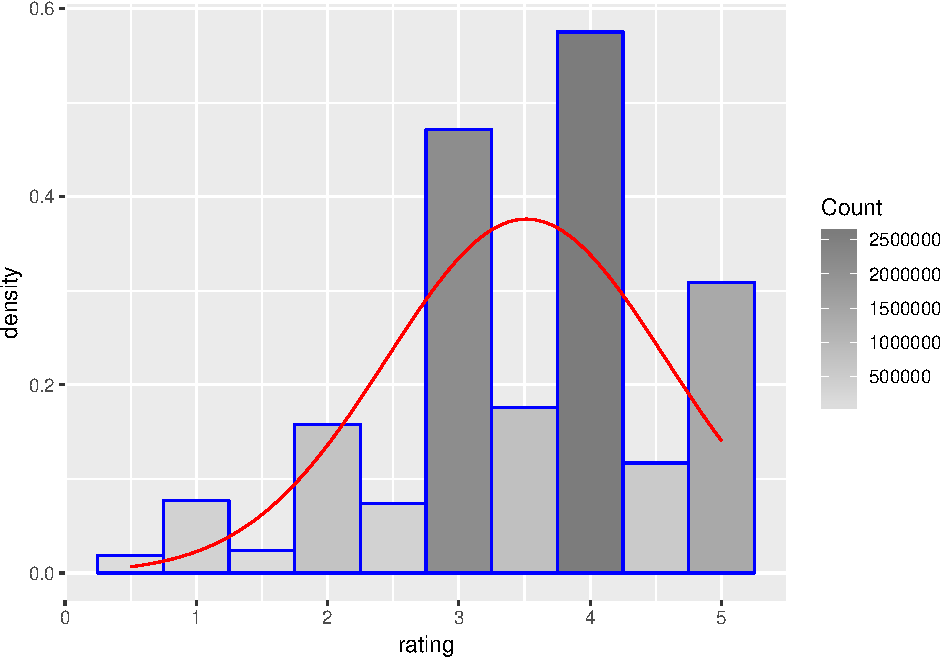
\includegraphics{Figs/unnamed-chunk-8-1.pdf}

The distribution is not really normal shaped and we see a negative
skewness. There is also no rating with the value 0 and most of the
ratings comes exactly at 3 and 4. Why there are more good ratings than
bad ones? This could be explained by the fact that when a user watch a
movie and like it, he finds the time to rate this movie. But when a user
does not like a movie, he simply doesn't bother and pass.

Now let's see how the number of ratings evolve with the release year of
the movies:

\begin{Shaded}
\begin{Highlighting}[]
\NormalTok{edx }\OperatorTok\StringTok{ }\KeywordTok{ggplot}\NormalTok{(}\KeywordTok{aes}\NormalTok{(year)) }\OperatorTok{+}
\StringTok{  }\KeywordTok{geom_histogram}\NormalTok{(}\DataTypeTok{fill =} \StringTok{"black"}\NormalTok{) }\OperatorTok{+}
\StringTok{  }\KeywordTok{labs}\NormalTok{(}\DataTypeTok{title =} \StringTok{"Frequency of ratings by relase year"}\NormalTok{,}
       \DataTypeTok{x =} \StringTok{"Year"}\NormalTok{,}
       \DataTypeTok{y =} \StringTok{"Frequency"}\NormalTok{)}
\end{Highlighting}
\end{Shaded}

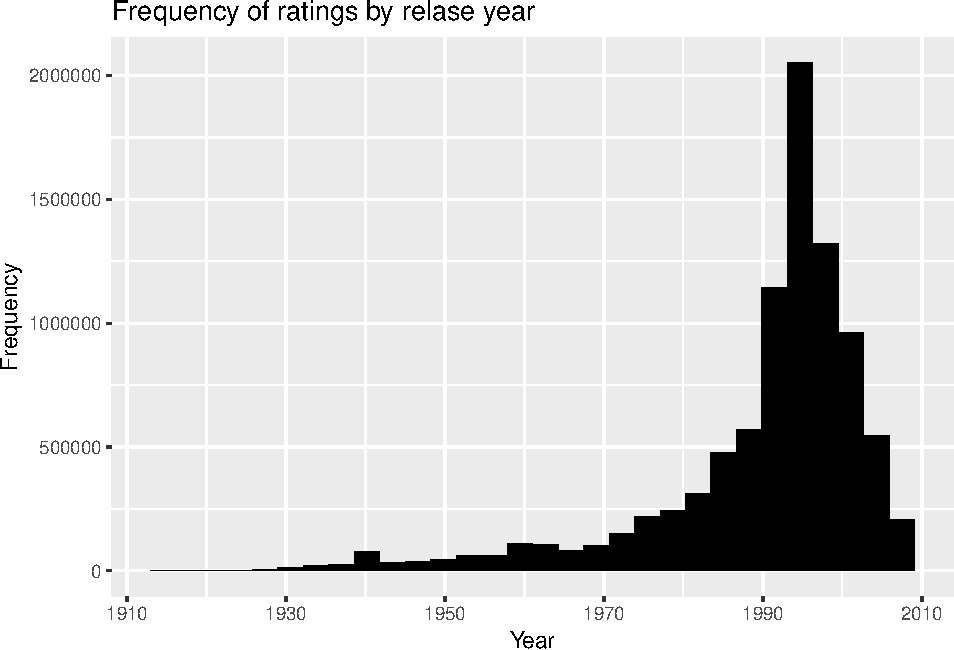
\includegraphics{Figs/unnamed-chunk-9-1.pdf}

Again we have a left skewed distribution with most of the ratings
happening between 1980 and 2009. Now let's introduce the age variable
and see its distribution:

\begin{Shaded}
\begin{Highlighting}[]
\NormalTok{edx <-}\StringTok{ }\NormalTok{edx }\OperatorTok\StringTok{ }\KeywordTok{mutate}\NormalTok{(}\DataTypeTok{age =}\NormalTok{ year_rate }\OperatorTok{-}\StringTok{ }\NormalTok{year)}

\NormalTok{plot1 <-}\StringTok{ }\NormalTok{edx }\OperatorTok\StringTok{ }\KeywordTok{ggplot}\NormalTok{(}\KeywordTok{aes}\NormalTok{(age)) }\OperatorTok{+}
\StringTok{  }\KeywordTok{geom_histogram}\NormalTok{(}\DataTypeTok{binwidth =} \DecValTok{5}\NormalTok{, }\DataTypeTok{fill =} \StringTok{"black"}\NormalTok{) }\OperatorTok{+}
\StringTok{  }\KeywordTok{labs}\NormalTok{(}\DataTypeTok{title =} \StringTok{"Frequency of ratings by age of the movie"}\NormalTok{,}
       \DataTypeTok{x =} \StringTok{"Age"}\NormalTok{,}
       \DataTypeTok{y =} \StringTok{"Frequency"}\NormalTok{)}

\NormalTok{plot2 <-}\StringTok{ }\NormalTok{edx }\OperatorTok\StringTok{ }
\StringTok{  }\KeywordTok{group_by}\NormalTok{(age) }\OperatorTok\StringTok{ }
\StringTok{  }\KeywordTok{summarize}\NormalTok{(}\DataTypeTok{b_a =} \KeywordTok{mean}\NormalTok{(rating)) }\OperatorTok\StringTok{ }
\StringTok{  }\KeywordTok{ggplot}\NormalTok{(}\KeywordTok{aes}\NormalTok{(b_a)) }\OperatorTok{+}\StringTok{ }
\StringTok{  }\KeywordTok{geom_histogram}\NormalTok{(}\DataTypeTok{color =} \StringTok{"darkblue"}\NormalTok{) }\OperatorTok{+}
\StringTok{  }\KeywordTok{ggtitle}\NormalTok{(}\StringTok{"Mean rating by age of the movie"}\NormalTok{)}

\KeywordTok{grid.arrange}\NormalTok{(plot1, plot2, }\DataTypeTok{ncol=}\DecValTok{2}\NormalTok{)}
\end{Highlighting}
\end{Shaded}

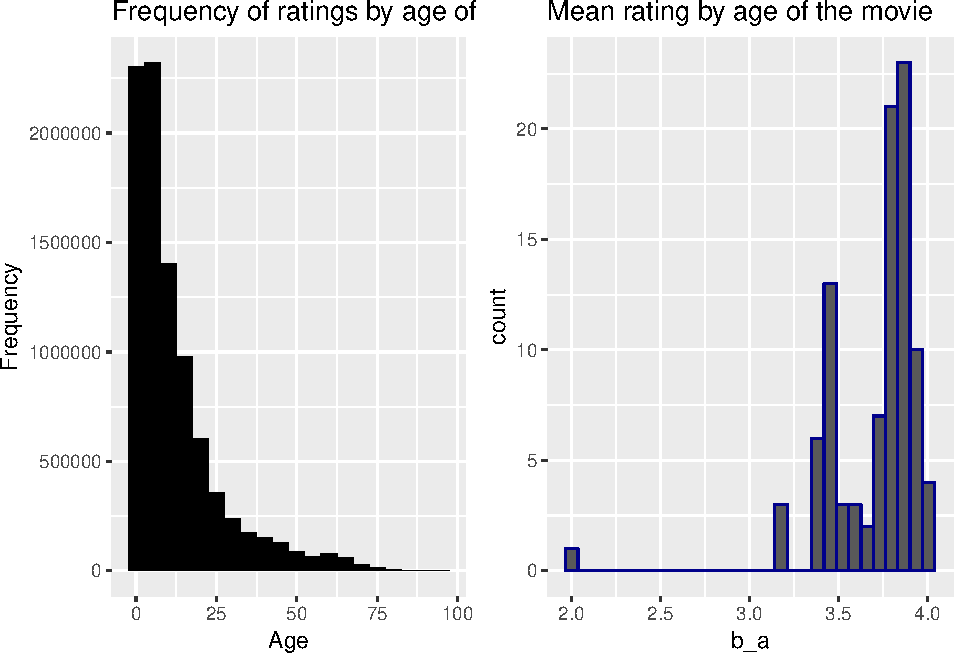
\includegraphics{Figs/unnamed-chunk-10-1.pdf}

The histogram explains that recent movies are rated more enough than
older ones. This can be explained by the fact that people tend to watch
popular movies and searching for new movies each time. People are
usually not very interested in old movies because either they have
watched many mavies before they started ratings movies or no one in
their social network recommands an old movie.

Now let's see if the users and the movies have some effect on the
ratings:

\begin{Shaded}
\begin{Highlighting}[]
\NormalTok{plot1 <-}\StringTok{ }\NormalTok{edx }\OperatorTok\StringTok{ }
\NormalTok{dplyr}\OperatorTok{::}\KeywordTok{count}\NormalTok{(userId) }\OperatorTok\StringTok{ }
\StringTok{  }\KeywordTok{ggplot}\NormalTok{(}\KeywordTok{aes}\NormalTok{(n)) }\OperatorTok{+}\StringTok{ }
\StringTok{  }\KeywordTok{geom_histogram}\NormalTok{(}\DataTypeTok{bins =} \DecValTok{30}\NormalTok{, }\DataTypeTok{color =} \StringTok{"black"}\NormalTok{) }\OperatorTok{+}\StringTok{ }
\StringTok{  }\KeywordTok{scale_x_log10}\NormalTok{() }\OperatorTok{+}\StringTok{ }
\StringTok{  }\KeywordTok{ggtitle}\NormalTok{(}\StringTok{"Rating count by users"}\NormalTok{)}
\NormalTok{plot2 <-}\StringTok{ }\NormalTok{edx }\OperatorTok\StringTok{ }
\StringTok{  }\KeywordTok{group_by}\NormalTok{(userId) }\OperatorTok\StringTok{ }
\StringTok{  }\KeywordTok{summarize}\NormalTok{(}\DataTypeTok{b_u =} \KeywordTok{mean}\NormalTok{(rating)) }\OperatorTok\StringTok{ }
\StringTok{  }\KeywordTok{filter}\NormalTok{(}\KeywordTok{n}\NormalTok{()}\OperatorTok{>=}\DecValTok{100}\NormalTok{) }\OperatorTok
\StringTok{  }\KeywordTok{ggplot}\NormalTok{(}\KeywordTok{aes}\NormalTok{(b_u)) }\OperatorTok{+}\StringTok{ }
\StringTok{  }\KeywordTok{geom_histogram}\NormalTok{(}\DataTypeTok{bins =} \DecValTok{30}\NormalTok{, }\DataTypeTok{color =} \StringTok{"darkblue"}\NormalTok{) }\OperatorTok{+}
\StringTok{  }\KeywordTok{ggtitle}\NormalTok{(}\StringTok{"Mean rating by users"}\NormalTok{)}
\NormalTok{plot3 <-}\StringTok{ }\NormalTok{edx }\OperatorTok\StringTok{ }
\StringTok{  }\NormalTok{dplyr}\OperatorTok{::}\KeywordTok{count}\NormalTok{(movieId) }\OperatorTok\StringTok{ }
\StringTok{  }\KeywordTok{ggplot}\NormalTok{(}\KeywordTok{aes}\NormalTok{(n)) }\OperatorTok{+}\StringTok{ }
\StringTok{  }\KeywordTok{geom_histogram}\NormalTok{(}\DataTypeTok{bins =} \DecValTok{30}\NormalTok{, }\DataTypeTok{color =} \StringTok{"black"}\NormalTok{) }\OperatorTok{+}\StringTok{ }
\StringTok{  }\KeywordTok{scale_x_log10}\NormalTok{() }\OperatorTok{+}\StringTok{ }
\StringTok{  }\KeywordTok{ggtitle}\NormalTok{(}\StringTok{"Rating count by movies"}\NormalTok{)}
\NormalTok{plot4 <-}\StringTok{ }\NormalTok{edx }\OperatorTok\StringTok{ }
\StringTok{  }\KeywordTok{group_by}\NormalTok{(userId) }\OperatorTok\StringTok{ }
\StringTok{  }\KeywordTok{summarize}\NormalTok{(}\DataTypeTok{b_m =} \KeywordTok{mean}\NormalTok{(rating)) }\OperatorTok\StringTok{ }
\StringTok{  }\KeywordTok{filter}\NormalTok{(}\KeywordTok{n}\NormalTok{()}\OperatorTok{>=}\DecValTok{100}\NormalTok{) }\OperatorTok
\StringTok{  }\KeywordTok{ggplot}\NormalTok{(}\KeywordTok{aes}\NormalTok{(b_m)) }\OperatorTok{+}\StringTok{ }
\StringTok{  }\KeywordTok{geom_histogram}\NormalTok{(}\DataTypeTok{bins =} \DecValTok{30}\NormalTok{, }\DataTypeTok{color =} \StringTok{"darkblue"}\NormalTok{) }\OperatorTok{+}
\StringTok{  }\KeywordTok{ggtitle}\NormalTok{(}\StringTok{"Mean rating by movies"}\NormalTok{)}
\KeywordTok{grid.arrange}\NormalTok{(plot1, plot2, plot3, plot4, }\DataTypeTok{ncol=}\DecValTok{2}\NormalTok{, }\DataTypeTok{nrow=}\DecValTok{2}\NormalTok{)}
\end{Highlighting}
\end{Shaded}

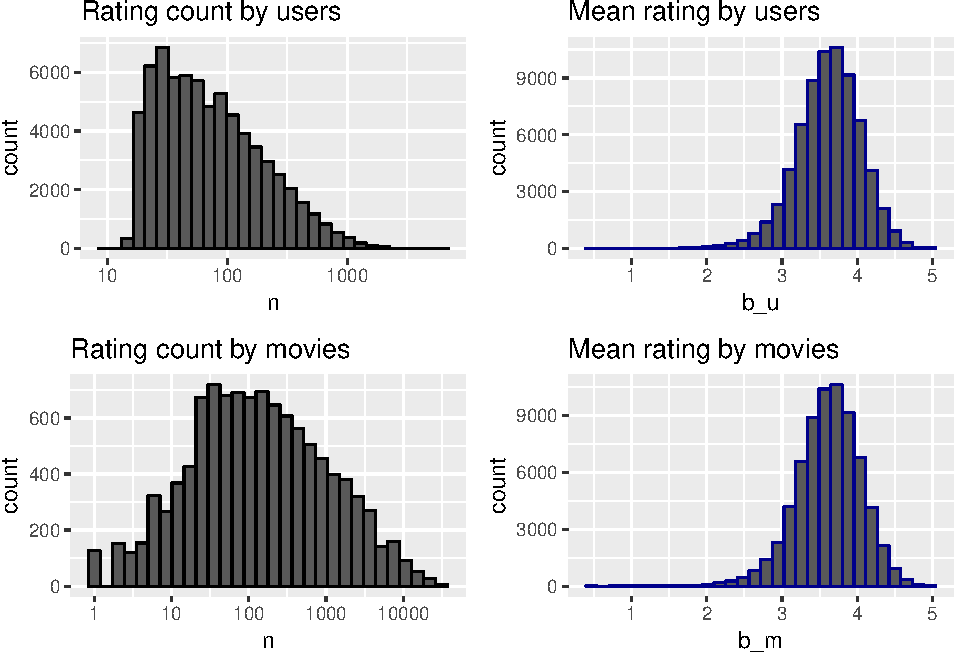
\includegraphics{Figs/unnamed-chunk-11-1.pdf}

Let's discuss the first row of the facet plot: we see that some users
are more active than others, some users are very cranky and others love
every movie. The same analysis applies for movies: some movies are rated
and appreciated more than others. This makes the variables users, movies
and age have a strong impact on the ratings.

Finally, let's print the genres and their corresponding average rating
by descending order to introduce a technique that will be relevant in
our modeling:

\begin{Shaded}
\begin{Highlighting}[]
\NormalTok{edx }\OperatorTok
\StringTok{  }\KeywordTok{select}\NormalTok{(genres, rating) }\OperatorTok
\StringTok{  }\KeywordTok{group_by}\NormalTok{(genres) }\OperatorTok
\StringTok{  }\KeywordTok{summarize}\NormalTok{(}\DataTypeTok{mean =} \KeywordTok{mean}\NormalTok{(rating), }\DataTypeTok{median =} \KeywordTok{median}\NormalTok{(rating), }\DataTypeTok{n =} \KeywordTok{n}\NormalTok{()) }\OperatorTok
\StringTok{  }\KeywordTok{arrange}\NormalTok{(}\KeywordTok{desc}\NormalTok{(mean)) }\OperatorTok
\StringTok{  }\KeywordTok{head}\NormalTok{(}\DecValTok{10}\NormalTok{)}
\end{Highlighting}
\end{Shaded}

\begin{verbatim}
## # A tibble: 10 x 4
##    genres                                   mean median     n
##    <fct>                                   <dbl>  <dbl> <int>
##  1 Animation|IMAX|Sci-Fi                    4.71    5       7
##  2 Drama|Film-Noir|Romance                  4.30    4.5  2989
##  3 Action|Crime|Drama|IMAX                  4.30    4.5  2353
##  4 Animation|Children|Comedy|Crime          4.28    4.5  7167
##  5 Film-Noir|Mystery                        4.24    4    5988
##  6 Crime|Film-Noir|Mystery                  4.22    4    4029
##  7 Film-Noir|Romance|Thriller               4.22    4    2453
##  8 Crime|Film-Noir|Thriller                 4.21    4    4844
##  9 Crime|Mystery|Thriller                   4.20    4   26892
## 10 Action|Adventure|Comedy|Fantasy|Romance  4.20    4   14809
\end{verbatim}

In this table, the genre ``Animation\textbar{}IMAX\textbar{}Sci-Fi'' has
the highest mean and median rating but this is not significant because
it only has 7 ratings. To deal with this problem, we introduce
regularization which permits us to penalize large estimates that are
formed using small sample sizes.

\section{Constructing the models}\label{constructing-the-models}

\subsection{1- Evaluation metric: loss function
(RMSE)}\label{evaluation-metric-loss-function-rmse}

In the NETFLIX challenge, they used the residual mean squared error to
evaluate the participant's models on a test set. Let's define
\(Y_{u,i}\) as the rating of movie i by user u and \(\hat{Y}_{u,i}\) as
the estimate of the same variable. The RMSE is formulated as follow:
\[RMSE = \frac{1}{N}\sum_{u,i}\left(\hat{Y}_{u,i} - Y_{u,i}\right)^2\]
with N being the number of user/movie combinations and the sum occurring
over all these combinations.

The RMSE is similar to a standard deviation. If a prediction model has
an RMSE larger than 1, this simply means that our errors are typically
far from the true rating by more than 1 star and this is not good since
1 constitute a big interval considering ratings from 0 to 5.

In the next sections, we will try different models and report their RMSE
in the variable rmse\_results.

\subsection{2- Basic model}\label{basic-model}

The simplest model one can think of is predicting one single value to
every input. It can be any statistic but people tend to choose the
median and the mean. Of course we can choose to generate random ratings
but in general, random predictions are often evaluated negatively. A
model that assumes the same rating for all movies and users with all the
differences explained by random variation would look like this:
\[ Y_{u,i} = \mu + \epsilon_{u,i} \] with \(\epsilon_{u,i}\)
independent errors sampled from the same distribution centered at 0 and
\(\mu\) the ``true'' rating for all movies. The best estimator in this
case would be the mean of all the ratings.

Let's build this model and report its result:

\begin{Shaded}
\begin{Highlighting}[]
\CommentTok{#Predicting the average for all users and movies}
\NormalTok{mu_hat <-}\StringTok{ }\KeywordTok{mean}\NormalTok{(edx}\OperatorTok{$}\NormalTok{rating)}
\NormalTok{naive_rmse <-}\StringTok{ }\KeywordTok{rmse}\NormalTok{(validation}\OperatorTok{$}\NormalTok{rating, mu_hat)}
\NormalTok{naive_rmse}
\end{Highlighting}
\end{Shaded}

\begin{verbatim}
## [1] 1.061202
\end{verbatim}

\begin{Shaded}
\begin{Highlighting}[]
\CommentTok{# Creating a dataframe containing the rmse results of all methods}
\NormalTok{rmse_results <-}\StringTok{ }\KeywordTok{data_frame}\NormalTok{(}\DataTypeTok{method =} \StringTok{"Just the average"}\NormalTok{, }\DataTypeTok{RMSE =}\NormalTok{ naive_rmse)}
\end{Highlighting}
\end{Shaded}

With just the average, the model is very bad because we are making a
typical error of 1.0612018 stars. We will improve this model by adding
some of the variables that had a clear impact on the ratings.

\subsection{3- Including other variables in the
model}\label{including-other-variables-in-the-model}

In this model, we will incorporate the effect of the movie, the user and
their combination to see whether our score is improving.

\subsubsection{The movie effect model}\label{the-movie-effect-model}

This model will be formulated as:
\[ Y_{u,i} = \mu + b_i + \epsilon_{u,i} \] where \(b_i\) is the average
of the difference between the movie rating and the global mean rating.

\begin{Shaded}
\begin{Highlighting}[]
\CommentTok{#first, estimate the effect of each movie bi}
\NormalTok{validation}\OperatorTok{$}\NormalTok{movieId <-}\StringTok{ }\KeywordTok{as.factor}\NormalTok{(validation}\OperatorTok{$}\NormalTok{movieId) }
\NormalTok{mu <-}\StringTok{ }\KeywordTok{mean}\NormalTok{(edx}\OperatorTok{$}\NormalTok{rating) }
\NormalTok{movie_avgs <-}\StringTok{ }\NormalTok{edx }\OperatorTok\StringTok{ }
\StringTok{  }\KeywordTok{group_by}\NormalTok{(movieId) }\OperatorTok\StringTok{ }
\StringTok{  }\KeywordTok{summarize}\NormalTok{(}\DataTypeTok{b_i =} \KeywordTok{mean}\NormalTok{(rating }\OperatorTok{-}\StringTok{ }\NormalTok{mu))}
\CommentTok{# then, make the prediction using the new model y= mu + b}
\NormalTok{predicted_ratings <-}\StringTok{ }\NormalTok{mu }\OperatorTok{+}\StringTok{ }\NormalTok{validation }\OperatorTok\StringTok{ }
\StringTok{  }\KeywordTok{left_join}\NormalTok{(movie_avgs, }\DataTypeTok{by=}\StringTok{'movieId'}\NormalTok{) }\OperatorTok
\StringTok{  }\NormalTok{.}\OperatorTok{$}\NormalTok{b_i}
\NormalTok{model_1_rmse <-}\StringTok{ }\KeywordTok{rmse}\NormalTok{(predicted_ratings, validation}\OperatorTok{$}\NormalTok{rating)}
\NormalTok{model_1_rmse}
\end{Highlighting}
\end{Shaded}

\begin{verbatim}
## [1] 0.9439087
\end{verbatim}

\begin{Shaded}
\begin{Highlighting}[]
\CommentTok{# Add the rmse result of the new model to the rmse data frame}
\NormalTok{rmse_results <-}\StringTok{ }\KeywordTok{bind_rows}\NormalTok{(rmse_results,}
                          \KeywordTok{data_frame}\NormalTok{(}\DataTypeTok{method=}\StringTok{"Movie Effect Model"}\NormalTok{,  }
                                     \DataTypeTok{RMSE =}\NormalTok{ model_1_rmse ))}
\end{Highlighting}
\end{Shaded}

\subsubsection{The user effect model}\label{the-user-effect-model}

This model will be formulated as:
\[ Y_{u,i} = \mu + b_u + \epsilon_{u,i} \] where \(b_u\) is the average
of the difference between the user rating and global mean rating \(\mu\)

\begin{Shaded}
\begin{Highlighting}[]
\CommentTok{#first, estimate the effect of each movie bi}
\NormalTok{mu <-}\StringTok{ }\KeywordTok{mean}\NormalTok{(edx}\OperatorTok{$}\NormalTok{rating) }
\NormalTok{users_avgs <-}\StringTok{ }\NormalTok{edx }\OperatorTok\StringTok{ }
\StringTok{  }\KeywordTok{group_by}\NormalTok{(userId) }\OperatorTok\StringTok{ }
\StringTok{  }\KeywordTok{summarize}\NormalTok{(}\DataTypeTok{b_u =} \KeywordTok{mean}\NormalTok{(rating }\OperatorTok{-}\StringTok{ }\NormalTok{mu))}
\CommentTok{# then, make the prediction using the new model y= mu + b}
\NormalTok{predicted_ratings <-}\StringTok{ }\NormalTok{mu }\OperatorTok{+}\StringTok{ }\NormalTok{validation }\OperatorTok\StringTok{ }
\StringTok{  }\KeywordTok{left_join}\NormalTok{(users_avgs, }\DataTypeTok{by=}\StringTok{'userId'}\NormalTok{) }\OperatorTok
\StringTok{  }\NormalTok{.}\OperatorTok{$}\NormalTok{b_u}
\NormalTok{model_2_rmse <-}\StringTok{ }\KeywordTok{rmse}\NormalTok{(predicted_ratings, validation}\OperatorTok{$}\NormalTok{rating)}
\NormalTok{model_2_rmse}
\end{Highlighting}
\end{Shaded}

\begin{verbatim}
## [1] 0.978336
\end{verbatim}

\begin{Shaded}
\begin{Highlighting}[]
\CommentTok{# Add the rmse result of the new model to the rmse data frame}
\NormalTok{rmse_results <-}\StringTok{ }\KeywordTok{bind_rows}\NormalTok{(rmse_results,}
                          \KeywordTok{data_frame}\NormalTok{(}\DataTypeTok{method=}\StringTok{"User Effect Model"}\NormalTok{,  }
                                     \DataTypeTok{RMSE =}\NormalTok{ model_2_rmse ))}
\end{Highlighting}
\end{Shaded}

\subsubsection{The movie and user effect
model}\label{the-movie-and-user-effect-model}

This model will be formulated as:
\[ Y_{u,i} = \mu + b_i +b_a + \epsilon_{u,i} \] where \(b_a\) is the
average of the difference between the user rating and the sum of the
global mean rating \(\mu\) and \(b_i\)

\begin{Shaded}
\begin{Highlighting}[]
\NormalTok{mvuser_avgs <-}\StringTok{ }\NormalTok{edx }\OperatorTok\StringTok{ }
\StringTok{  }\KeywordTok{left_join}\NormalTok{(movie_avgs, }\DataTypeTok{by=}\StringTok{'movieId'}\NormalTok{) }\OperatorTok
\StringTok{  }\KeywordTok{group_by}\NormalTok{(userId) }\OperatorTok
\StringTok{  }\KeywordTok{summarize}\NormalTok{(}\DataTypeTok{b_a =} \KeywordTok{mean}\NormalTok{(rating }\OperatorTok{-}\StringTok{ }\NormalTok{mu }\OperatorTok{-}\StringTok{ }\NormalTok{b_i))}
\CommentTok{# Now, compute the predicted ratings using the new model with user and movie effects:}
\NormalTok{predicted_ratings <-}\StringTok{ }\NormalTok{validation }\OperatorTok\StringTok{ }
\StringTok{  }\KeywordTok{left_join}\NormalTok{(movie_avgs, }\DataTypeTok{by=}\StringTok{'movieId'}\NormalTok{) }\OperatorTok
\StringTok{  }\KeywordTok{left_join}\NormalTok{(mvuser_avgs, }\DataTypeTok{by=}\StringTok{'userId'}\NormalTok{) }\OperatorTok
\StringTok{  }\KeywordTok{mutate}\NormalTok{(}\DataTypeTok{pred =}\NormalTok{ mu }\OperatorTok{+}\StringTok{ }\NormalTok{b_i }\OperatorTok{+}\StringTok{ }\NormalTok{b_a) }\OperatorTok
\StringTok{  }\NormalTok{.}\OperatorTok{$}\NormalTok{pred}
\NormalTok{model_3_rmse <-}\StringTok{ }\KeywordTok{RMSE}\NormalTok{(predicted_ratings, validation}\OperatorTok{$}\NormalTok{rating)}
\NormalTok{model_3_rmse}
\end{Highlighting}
\end{Shaded}

\begin{verbatim}
## [1] 0.8653488
\end{verbatim}

\begin{Shaded}
\begin{Highlighting}[]
\CommentTok{# Add the rmse result of the new model to the rmse data frame}
\NormalTok{rmse_results <-}\StringTok{ }\KeywordTok{bind_rows}\NormalTok{(rmse_results,}
                          \KeywordTok{data_frame}\NormalTok{(}\DataTypeTok{method=}\StringTok{"Movie + User Effects Model"}\NormalTok{,  }
                                     \DataTypeTok{RMSE =}\NormalTok{ model_3_rmse ))}
\end{Highlighting}
\end{Shaded}

\subsubsection{The movie, user and age effect
model}\label{the-movie-user-and-age-effect-model}

This model will be formulated as:
\[ Y_{u,i} = \mu + b_i +b_a + b_g + \epsilon_{u,i} \] where \(b_g\) is
the average of the difference between the age rating and the sum of the
global mean rating \(\mu\), \(b_i\) and \(b_a\)

\begin{Shaded}
\begin{Highlighting}[]
\CommentTok{# Let's compute the new term bu in our mode y= mu+bi+ba+bg +eps}
\NormalTok{age_avgs <-}\StringTok{ }\NormalTok{edx }\OperatorTok\StringTok{ }
\StringTok{  }\KeywordTok{left_join}\NormalTok{(movie_avgs, }\DataTypeTok{by=}\StringTok{'movieId'}\NormalTok{) }\OperatorTok
\StringTok{  }\KeywordTok{left_join}\NormalTok{(mvuser_avgs, }\DataTypeTok{by=}\StringTok{'userId'}\NormalTok{) }\OperatorTok
\StringTok{  }\KeywordTok{group_by}\NormalTok{(age) }\OperatorTok
\StringTok{  }\KeywordTok{summarize}\NormalTok{(}\DataTypeTok{b_g =} \KeywordTok{mean}\NormalTok{(rating }\OperatorTok{-}\StringTok{ }\NormalTok{mu }\OperatorTok{-}\StringTok{ }\NormalTok{b_i }\OperatorTok{-}\StringTok{ }\NormalTok{b_a))}

\CommentTok{# process the variable age so that leftjoin finds values in LHS}
\NormalTok{listofages <-}\StringTok{ }\KeywordTok{unique}\NormalTok{(age_avgs}\OperatorTok{$}\NormalTok{age)}
\NormalTok{ages <-}\StringTok{ }\NormalTok{validation}\OperatorTok{$}\NormalTok{age}
\NormalTok{validation}\OperatorTok{$}\NormalTok{age <-}\StringTok{ }\KeywordTok{sapply}\NormalTok{(ages, }\ControlFlowTok{function}\NormalTok{(x)\{ listofages[}\KeywordTok{which.min}\NormalTok{(}\KeywordTok{abs}\NormalTok{(listofages}\OperatorTok{-}\NormalTok{x))]\})}
\CommentTok{# Now, compute the predicted ratings using the new model with user and movie effects:}
\NormalTok{predicted_ratings <-}\StringTok{ }\NormalTok{validation }\OperatorTok\StringTok{ }
\StringTok{  }\KeywordTok{left_join}\NormalTok{(movie_avgs, }\DataTypeTok{by=}\StringTok{'movieId'}\NormalTok{) }\OperatorTok
\StringTok{  }\KeywordTok{left_join}\NormalTok{(mvuser_avgs, }\DataTypeTok{by=}\StringTok{'userId'}\NormalTok{) }\OperatorTok
\StringTok{  }\KeywordTok{left_join}\NormalTok{(age_avgs, }\DataTypeTok{by=}\StringTok{'age'}\NormalTok{) }\OperatorTok
\StringTok{  }\KeywordTok{mutate}\NormalTok{(}\DataTypeTok{pred =}\NormalTok{ mu }\OperatorTok{+}\StringTok{ }\NormalTok{b_i }\OperatorTok{+}\StringTok{ }\NormalTok{b_a }\OperatorTok{+}\StringTok{ }\NormalTok{b_g) }\OperatorTok
\StringTok{  }\NormalTok{.}\OperatorTok{$}\NormalTok{pred}
\NormalTok{model_4_rmse <-}\StringTok{ }\KeywordTok{RMSE}\NormalTok{(predicted_ratings, validation}\OperatorTok{$}\NormalTok{rating)}
\NormalTok{model_4_rmse}
\end{Highlighting}
\end{Shaded}

\begin{verbatim}
## [1] 0.8649038
\end{verbatim}

\begin{Shaded}
\begin{Highlighting}[]
\CommentTok{# Add the rmse result of the new model to the rmse data frame}
\NormalTok{rmse_results <-}\StringTok{ }\KeywordTok{bind_rows}\NormalTok{(rmse_results,}
                          \KeywordTok{data_frame}\NormalTok{(}\DataTypeTok{method=}\StringTok{"Movie + User + Age Effects Model"}\NormalTok{,  }
                                     \DataTypeTok{RMSE =}\NormalTok{ model_4_rmse ))}
\end{Highlighting}
\end{Shaded}

\subsubsection{Using regularization to improve the
score}\label{using-regularization-to-improve-the-score}

The rmse results up to now are still not very good. Maybe we are making
some errors in our predictions. To make sure, let's take the first model
(movie effect) and print the movies with the best ratings:

\begin{Shaded}
\begin{Highlighting}[]
\NormalTok{save_edx}\OperatorTok{$}\NormalTok{movieId <-}\StringTok{ }\KeywordTok{as.factor}\NormalTok{(save_edx}\OperatorTok{$}\NormalTok{movieId)}

\NormalTok{movie_titles <-}\StringTok{ }\NormalTok{save_edx }\OperatorTok\StringTok{ }
\StringTok{  }\KeywordTok{select}\NormalTok{(movieId, title) }\OperatorTok
\StringTok{  }\KeywordTok{distinct}\NormalTok{()}

\NormalTok{save_edx }\OperatorTok\StringTok{ }\NormalTok{dplyr}\OperatorTok{::}\KeywordTok{count}\NormalTok{(movieId) }\OperatorTok\StringTok{ }
\StringTok{  }\KeywordTok{left_join}\NormalTok{(movie_avgs, }\DataTypeTok{by=}\StringTok{"movieId"}\NormalTok{) }\OperatorTok
\StringTok{  }\KeywordTok{left_join}\NormalTok{(movie_titles, }\DataTypeTok{by=}\StringTok{"movieId"}\NormalTok{) }\OperatorTok
\StringTok{  }\KeywordTok{arrange}\NormalTok{(}\KeywordTok{desc}\NormalTok{(b_i)) }\OperatorTok\StringTok{ }
\StringTok{  }\KeywordTok{select}\NormalTok{(title, b_i, n) }\OperatorTok\StringTok{ }
\StringTok{  }\KeywordTok{slice}\NormalTok{(}\DecValTok{1}\OperatorTok{:}\DecValTok{10}\NormalTok{)}
\end{Highlighting}
\end{Shaded}

\begin{verbatim}
## # A tibble: 10 x 3
##    title                                                          b_i     n
##    <chr>                                                        <dbl> <int>
##  1 Hellhounds on My Trail (1999)                                 1.49     1
##  2 "Satan's Tango (S\u00e1t\u00e1ntang\u00f3) (1994)"            1.49     2
##  3 Shadows of Forgotten Ancestors (1964)                         1.49     1
##  4 Fighting Elegy (Kenka erejii) (1966)                          1.49     1
##  5 Sun Alley (Sonnenallee) (1999)                                1.49     1
##  6 Blue Light, The (Das Blaue Licht) (1932)                      1.49     1
##  7 Who's Singin' Over There? (a.k.a. Who Sings Over There) (Ko~  1.24     4
##  8 Human Condition II, The (Ningen no joken II) (1959)           1.24     4
##  9 Human Condition III, The (Ningen no joken III) (1961)         1.24     4
## 10 Constantine's Sword (2007)                                    1.24     2
\end{verbatim}

We see that those movies were only rated by a very few users so our
mispredictions comes from this small samples. We can deal with those
errors by introducing regularization. The general idea behind it is to
constrain the total variability of the effect sizes by adding a penalty
term to the least square equation, that gets larger when \(b_i\) are
large. The penalty term is a parameter that should be tuned to optimise
the objective.

\begin{Shaded}
\begin{Highlighting}[]
\CommentTok{# Using regularization and tuning the penalty term}

\NormalTok{lambdas <-}\StringTok{ }\KeywordTok{seq}\NormalTok{(}\DecValTok{0}\NormalTok{, }\DecValTok{10}\NormalTok{, }\FloatTok{0.25}\NormalTok{)}

\NormalTok{rmses <-}\StringTok{ }\KeywordTok{sapply}\NormalTok{(lambdas, }\ControlFlowTok{function}\NormalTok{(l)\{}
  
\NormalTok{  mu <-}\StringTok{ }\KeywordTok{mean}\NormalTok{(edx}\OperatorTok{$}\NormalTok{rating)}
  
\NormalTok{  b_i <-}\StringTok{ }\NormalTok{edx }\OperatorTok\StringTok{ }
\StringTok{    }\KeywordTok{group_by}\NormalTok{(movieId) }\OperatorTok
\StringTok{    }\KeywordTok{summarize}\NormalTok{(}\DataTypeTok{b_i =} \KeywordTok{sum}\NormalTok{(rating }\OperatorTok{-}\StringTok{ }\NormalTok{mu)}\OperatorTok{/}\NormalTok{(}\KeywordTok{n}\NormalTok{()}\OperatorTok{+}\NormalTok{l))}
  
\NormalTok{  b_a <-}\StringTok{ }\NormalTok{edx }\OperatorTok\StringTok{ }
\StringTok{    }\KeywordTok{left_join}\NormalTok{(b_i, }\DataTypeTok{by=}\StringTok{"movieId"}\NormalTok{) }\OperatorTok
\StringTok{    }\KeywordTok{group_by}\NormalTok{(userId) }\OperatorTok
\StringTok{    }\KeywordTok{summarize}\NormalTok{(}\DataTypeTok{b_a =} \KeywordTok{sum}\NormalTok{(rating }\OperatorTok{-}\StringTok{ }\NormalTok{b_i }\OperatorTok{-}\StringTok{ }\NormalTok{mu)}\OperatorTok{/}\NormalTok{(}\KeywordTok{n}\NormalTok{()}\OperatorTok{+}\NormalTok{l))}
  
\NormalTok{  b_g <-}\StringTok{ }\NormalTok{edx }\OperatorTok\StringTok{ }
\StringTok{    }\KeywordTok{left_join}\NormalTok{(b_i, }\DataTypeTok{by=}\StringTok{"movieId"}\NormalTok{) }\OperatorTok
\StringTok{    }\KeywordTok{left_join}\NormalTok{(b_a, }\DataTypeTok{by=}\StringTok{"userId"}\NormalTok{) }\OperatorTok
\StringTok{    }\KeywordTok{group_by}\NormalTok{(age)}\OperatorTok
\StringTok{    }\KeywordTok{summarize}\NormalTok{(}\DataTypeTok{b_g =} \KeywordTok{sum}\NormalTok{(rating }\OperatorTok{-}\StringTok{ }\NormalTok{b_i }\OperatorTok{-}\StringTok{ }\NormalTok{b_a }\OperatorTok{-}\StringTok{ }\NormalTok{mu)}\OperatorTok{/}\NormalTok{(}\KeywordTok{n}\NormalTok{()}\OperatorTok{+}\NormalTok{l))}
  
  
\NormalTok{  predicted_ratings <-}\StringTok{ }
\StringTok{    }\NormalTok{validation }\OperatorTok\StringTok{ }
\StringTok{    }\KeywordTok{left_join}\NormalTok{(b_i, }\DataTypeTok{by =} \StringTok{"movieId"}\NormalTok{) }\OperatorTok
\StringTok{    }\KeywordTok{left_join}\NormalTok{(b_a, }\DataTypeTok{by =} \StringTok{"userId"}\NormalTok{) }\OperatorTok
\StringTok{    }\KeywordTok{left_join}\NormalTok{(b_g, }\DataTypeTok{by =} \StringTok{"age"}\NormalTok{) }\OperatorTok
\StringTok{    }\KeywordTok{mutate}\NormalTok{(}\DataTypeTok{pred =}\NormalTok{ mu }\OperatorTok{+}\StringTok{ }\NormalTok{b_i }\OperatorTok{+}\StringTok{ }\NormalTok{b_a }\OperatorTok{+}\StringTok{ }\NormalTok{b_g) }\OperatorTok
\StringTok{    }\NormalTok{.}\OperatorTok{$}\NormalTok{pred}
  
  \KeywordTok{return}\NormalTok{(}\KeywordTok{rmse}\NormalTok{(predicted_ratings, validation}\OperatorTok{$}\NormalTok{rating))}
\NormalTok{\})}

\CommentTok{# Plot the values or RMSE against lambdas}
\KeywordTok{qplot}\NormalTok{(lambdas, rmses)}
\end{Highlighting}
\end{Shaded}

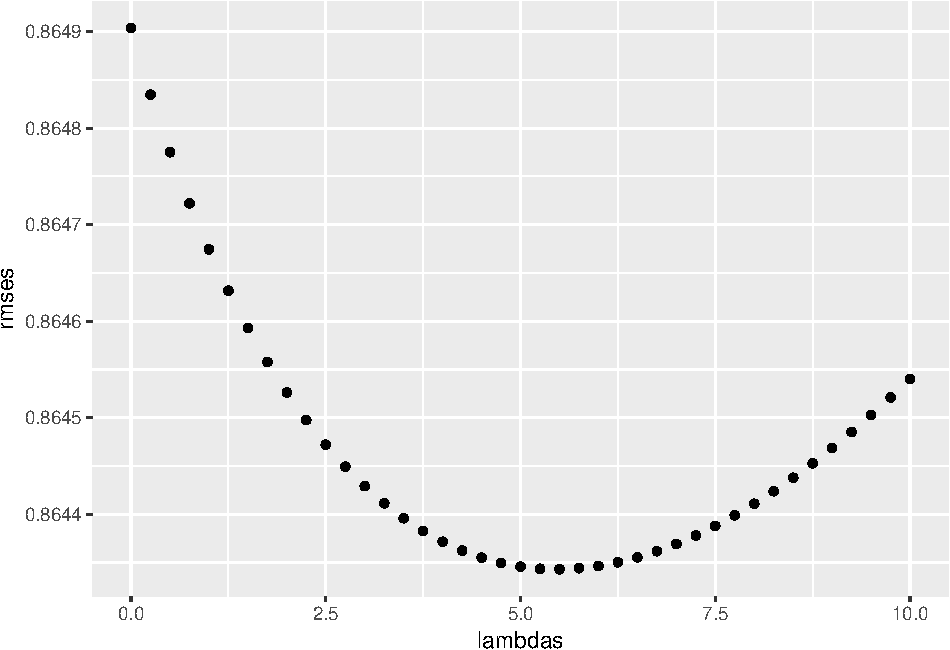
\includegraphics{Figs/unnamed-chunk-19-1.pdf}

\begin{Shaded}
\begin{Highlighting}[]
\CommentTok{# Find the value of lambda that minimizes the RMSE}
\NormalTok{lambdas[}\KeywordTok{which.min}\NormalTok{(rmses)]}
\end{Highlighting}
\end{Shaded}

\begin{verbatim}
## [1] 5.5
\end{verbatim}

\begin{Shaded}
\begin{Highlighting}[]
\KeywordTok{min}\NormalTok{(rmses)}
\end{Highlighting}
\end{Shaded}

\begin{verbatim}
## [1] 0.864343
\end{verbatim}

\begin{Shaded}
\begin{Highlighting}[]
\CommentTok{# save the model with the minimal RMSE to the results data frame}

\NormalTok{rmse_results <-}\StringTok{ }\KeywordTok{bind_rows}\NormalTok{(rmse_results,}
                          \KeywordTok{data_frame}\NormalTok{(}\DataTypeTok{method=}\StringTok{"Regularized Movie + User + age Effect Model"}\NormalTok{,  }
                                     \DataTypeTok{RMSE =} \KeywordTok{min}\NormalTok{(rmses)))}
\end{Highlighting}
\end{Shaded}

\section{Result discussion}\label{result-discussion}

In this section, we show our results for the five models we implemented:

\begin{Shaded}
\begin{Highlighting}[]
\NormalTok{rmse_results }\OperatorTok\StringTok{ }\NormalTok{knitr}\OperatorTok{::}\KeywordTok{kable}\NormalTok{(}\DataTypeTok{caption =} \StringTok{"Summary of the RMSEs"}\NormalTok{)}
\end{Highlighting}
\end{Shaded}

\begin{longtable}[]{@{}lr@{}}
\caption{Summary of the RMSEs}\tabularnewline
\toprule
method & RMSE\tabularnewline
\midrule
\endfirsthead
\toprule
method & RMSE\tabularnewline
\midrule
\endhead
Just the average & 1.0612018\tabularnewline
Movie Effect Model & 0.9439087\tabularnewline
User Effect Model & 0.9783360\tabularnewline
Movie + User Effects Model & 0.8653488\tabularnewline
Movie + User + Age Effects Model & 0.8649038\tabularnewline
Regularized Movie + User + age Effect Model & 0.8643430\tabularnewline
\bottomrule
\end{longtable}

As expected, all the models are better than the one value prediction
based on the average. The movieId variable had a strong impact on the
rmse and combining it with the usedId made the rmse smaller. The age
variable a very small impact comparing to the first two. The best rmse
0.864343 is then obtained by the last model

\section{Conclusion}\label{conclusion}

In this project, we had the chance to apply many of the techniques
learned in data exploration, visualization and machine learning courses.
We tried to get to an RMSE result below 0.87 and we achieved this
result. We can move forward and try new algorithms like matrix
factorization, gradient boosting machines, random forest on a larger
dataset. However, such work will certainly need more computation power.
We can try those techniques in a future work.

I would like to thank Professor Rafael A. Irizarry for this wonderful
and well detailed course on the edX plateforme. Special thanks for the
students who made all the problems clear and made the forums a
complementary learning space.


\end{document}
